\section{Graphentheorie}

Ein grundlegendes, strukturelles Verständniss von Graphen ist wichtig für diese Arbeit, da diese mathematische Struktur
die Grundlage der gesamten Arbeit bildet. In diesem Kapitel werden viele Definitionen mithilfe eines mathematischen
Lehrbuchs erarbeitet. Es wird später ersichtlich werden wozu diese Definitionen wichtig sind auch wenn diese jetzt noch
sehr abstrakt erscheinen.

\subsection{allgemeiner Graph}

Ein Graph ist ein Paar $\textrm{G = (V, E)}$ zweier disjunkter Mengen (vgl. Graphlehrbuch) mit E $\subseteq$ V^2 (vgl. Graphlehrbuch)

Elemente von V nennt man Knoten eines Graphens, die Elemente von E nennt man Kanten, Knoten die in einem Tupel von E vorkommen
nennt man auch inzident (benachbart).
Ein Graph könnte man nun definieren indem wir z.B. für V = {1, 2, 3} wählen und für E = {(1, 1), (1, 2), (1, 3)}.
Dargestellt werden können Graphen indem man die Elemente von V als z.B. Kreis zeichnet und dann alle Kanten aus E
einzeichnet indem man die Punkte verbindet. Eben definierter Graph hat z.B. folgende Darstellung:

\begin{center}
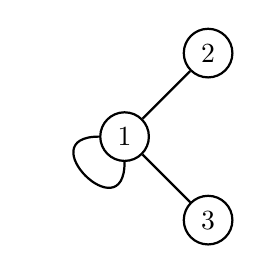
\begin{tikzpicture}[node distance={15mm}, thick, main/.style = {draw, circle}]
    \node[main] (1) {$1$};
    \node[main] (2) [above right of=1] {$2$};
    \node[main] (3) [below right of=1] {$3$};
    \draw (1) to [out=180,in=270,looseness=5] (1);
    \draw (1) -- (2);
    \draw (1) -- (3);
\end{tikzpicture}
\end{center}

Mit dieser Definition lassen sich nun beliebig große Graphen erstellen.
Einige Eigenschaften von Graphen müssen nun noch genau definiert werden da diese später relevant sein werden.
Zu definieren sind Wege und Kreise sowie die gerichtete Graphen

\subsection{Gerichteter Graph}

Im Kontext der Überdeckungskriterien sind gerichtete Graphen eher angewandt als ungerichtete, da diese durch ihre
Struktur den Programmfluss besser abbilden können.
Ein gerichteter Graph G ist definiert als:

\begin{description}
    \item[Menge N] von Knoten
    \item[Menge N_{0}] von Anfangsknoten, wobei N_{0} $\subseteq$ N
    \item[Menge N_{f}] von Endknoten, wobei N_{f} $\subseteq$ N
    \item[Menge E] von Kanten, wobei E $\subseteq$ N x N. Hierbei ist die Menge als init{x} x target{y} definiert.
\end{description} (vgl. Introduction to Softwaretesting 1-1 Kopie)

Im Grunde ist die Definition sehr ähnlich zu dem eines ungerichteten Graphen. Nur die Defintion der Kanten unterscheidet
sich. In einem ungerichteten Graphen hat die Kante (1,2) einen Weg von Knoten 1 zu Knoten 2 und umgedreht.
Wohingegen dieselbe Kante in einem gerichteten Graphen nur den Weg von Knoten 1 zu Knoten 2 hat.
Für das Beispiel von ungerichteten Graphen also V = {1, 2, 3} und E = {(1, 1), (1, 2), (1, 3)} ergibt sich also folgender Graph:

\begin{center}
    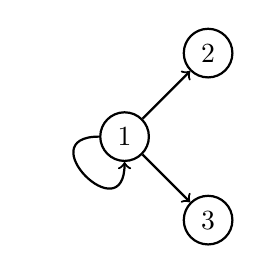
\begin{tikzpicture}[node distance={15mm}, thick, main/.style = {draw, circle}]
        \node[main] (1) {$1$};
        \node[main] (2) [above right of=1] {$2$};
        \node[main] (3) [below right of=1] {$3$};
        \draw[->] (1) to [out=180,in=270,looseness=5] (1);
        \draw[->] (1) to (2);
        \draw[->] (1) to (3);
    \end{tikzpicture}
\end{center}

\subsection{Wege und Kreise}
\subsubsection{Wege}
Ein Weg ist eine Sequenz [1,2,...,X] von Knoten, welche alle paarweise adjazent sind. (vgl. Software Testing Intro)

\subsubsection{Kreis}
Ein Kreis ist ein Weg bei dem Start und Endknoten identisch sind.

\subsection{Erreichbarkeit}
Ein Knoten ist erreichbar von einem anderen Knoten wenn ein Weg von einem zum anderen Knoten existiert.


